% Options for packages loaded elsewhere
\PassOptionsToPackage{unicode}{hyperref}
\PassOptionsToPackage{hyphens}{url}
%
\documentclass[
]{article}
\title{ISGC}
\author{Marion Maisonobe}
\date{30/04/2021}

\usepackage{amsmath,amssymb}
\usepackage{lmodern}
\usepackage{iftex}
\ifPDFTeX
  \usepackage[T1]{fontenc}
  \usepackage[utf8]{inputenc}
  \usepackage{textcomp} % provide euro and other symbols
\else % if luatex or xetex
  \usepackage{unicode-math}
  \defaultfontfeatures{Scale=MatchLowercase}
  \defaultfontfeatures[\rmfamily]{Ligatures=TeX,Scale=1}
\fi
% Use upquote if available, for straight quotes in verbatim environments
\IfFileExists{upquote.sty}{\usepackage{upquote}}{}
\IfFileExists{microtype.sty}{% use microtype if available
  \usepackage[]{microtype}
  \UseMicrotypeSet[protrusion]{basicmath} % disable protrusion for tt fonts
}{}
\makeatletter
\@ifundefined{KOMAClassName}{% if non-KOMA class
  \IfFileExists{parskip.sty}{%
    \usepackage{parskip}
  }{% else
    \setlength{\parindent}{0pt}
    \setlength{\parskip}{6pt plus 2pt minus 1pt}}
}{% if KOMA class
  \KOMAoptions{parskip=half}}
\makeatother
\usepackage{xcolor}
\IfFileExists{xurl.sty}{\usepackage{xurl}}{} % add URL line breaks if available
\IfFileExists{bookmark.sty}{\usepackage{bookmark}}{\usepackage{hyperref}}
\hypersetup{
  pdftitle={ISGC},
  pdfauthor={Marion Maisonobe},
  hidelinks,
  pdfcreator={LaTeX via pandoc}}
\urlstyle{same} % disable monospaced font for URLs
\usepackage[margin=1in]{geometry}
\usepackage{graphicx}
\makeatletter
\def\maxwidth{\ifdim\Gin@nat@width>\linewidth\linewidth\else\Gin@nat@width\fi}
\def\maxheight{\ifdim\Gin@nat@height>\textheight\textheight\else\Gin@nat@height\fi}
\makeatother
% Scale images if necessary, so that they will not overflow the page
% margins by default, and it is still possible to overwrite the defaults
% using explicit options in \includegraphics[width, height, ...]{}
\setkeys{Gin}{width=\maxwidth,height=\maxheight,keepaspectratio}
% Set default figure placement to htbp
\makeatletter
\def\fps@figure{htbp}
\makeatother
\setlength{\emergencystretch}{3em} % prevent overfull lines
\providecommand{\tightlist}{%
  \setlength{\itemsep}{0pt}\setlength{\parskip}{0pt}}
\setcounter{secnumdepth}{-\maxdimen} % remove section numbering
\usepackage{booktabs}
\usepackage{longtable}
\usepackage{array}
\usepackage{multirow}
\usepackage{wrapfig}
\usepackage{float}
\usepackage{colortbl}
\usepackage{pdflscape}
\usepackage{tabu}
\usepackage{threeparttable}
\usepackage{threeparttablex}
\usepackage[normalem]{ulem}
\usepackage{makecell}
\usepackage{xcolor}
\ifLuaTeX
  \usepackage{selnolig}  % disable illegal ligatures
\fi

\begin{document}
\maketitle

\hypertarget{isgc-congress}{%
\subsection{ISGC Congress}\label{isgc-congress}}

ISGC is an international conference of green chemistry held every two
years in La Rochelle since 2013. In the frame of the NETCONF research
project we focus on several editions of the conference in order to study
its structure and dynamics. we are interested in communications, panels,
topics, participants and their geographical origin. We consider studying
conferences can bring many insights on emergent scientific communities,
both regarding their organisation and dynamics.

\hypertarget{topics}{%
\subsection{Topics}\label{topics}}

We first look at the topics associated to flash and oral communications
given at the ISGC congress over time. We notice that Biomass conversion
is the more popular topic. It attracted 80 communications at the 2019
edition. However, we notice that certain topics are not represented at
every ISGC editions. It is notably the case of Biomass conversion which
was not present at the 2017 edition. During the 2017 edition, it appears
that Biomass conversion has been temporarily replaced by another
category named Renewable carbon (see Table 1 below).

\begin{table}
\centering
\begin{tabular}[t]{l|r|>{}r|r|>{}r|r|>{}r|r|>{}r}
\hline
\multicolumn{1}{c|}{ } & \multicolumn{8}{c}{Number and \% of oral and flash communications} \\
\cline{2-9}
\multicolumn{1}{c|}{ } & \multicolumn{2}{c|}{2015} & \multicolumn{2}{c|}{2017} & \multicolumn{2}{c|}{2019} & \multicolumn{2}{c}{Total} \\
\cline{2-3} \cline{4-5} \cline{6-7} \cline{8-9}
\multicolumn{1}{c|}{ISGC topic} & \multicolumn{1}{c|}{Nb} & \multicolumn{1}{c|}{\%} & \multicolumn{1}{c|}{Nb} & \multicolumn{1}{c|}{\%} & \multicolumn{1}{c|}{Nb} & \multicolumn{1}{c|}{\%} & \multicolumn{1}{c|}{Nb} & \multicolumn{1}{c}{\%} \\
\cline{1-1} \cline{2-2} \cline{3-3} \cline{4-4} \cline{5-5} \cline{6-6} \cline{7-7} \cline{8-8} \cline{9-9}
Biomass conversion & 93 & 38.3 & 0 & 0.0 & 80 & 26.0 & 173 & 20.2\\
\hline
Renewable carbon & 0 & \em{0.0} & 125 & \em{41.0} & 0 & \em{0.0} & 125 & \em{14.6}\\
\hline
Alternative solvents & 31 & \em{12.8} & 35 & \em{11.5} & 24 & \em{7.8} & 90 & \em{10.5}\\
\hline
Homogenous, heterogenous and biocatalysis & 0 & \em{0.0} & 0 & \em{0.0} & 68 & \em{22.1} & 68 & \em{7.9}\\
\hline
Polymers & 0 & \em{0.0} & 33 & \em{10.8} & 28 & \em{9.1} & 61 & \em{7.1}\\
\hline
Catalytic systems & 0 & \em{0.0} & 58 & \em{19.0} & 0 & \em{0.0} & 58 & \em{6.8}\\
\hline
Polymers and materials & 36 & \em{14.8} & 0 & \em{0.0} & 0 & \em{0.0} & 36 & \em{4.2}\\
\hline
Waste valorization & 0 & \em{0.0} & 0 & \em{0.0} & 34 & \em{11.0} & 34 & \em{4.0}\\
\hline
Alternative technologies & 0 & \em{0.0} & 0 & \em{0.0} & 24 & \em{7.8} & 24 & \em{2.8}\\
\hline
Atom-economy synthesis & 22 & \em{9.1} & 0 & \em{0.0} & 0 & \em{0.0} & 22 & \em{2.6}\\
\hline
Chemical valorization of wastes & 18 & \em{7.4} & 0 & \em{0.0} & 0 & \em{0.0} & 18 & \em{2.1}\\
\hline
Environnemental impact and life cycle assessment & 0 & \em{0.0} & 16 & \em{5.2} & 0 & \em{0.0} & 16 & \em{1.9}\\
\hline
Clean reactions & 0 & \em{0.0} & 0 & \em{0.0} & 16 & \em{5.2} & 16 & \em{1.9}\\
\hline
Eco-technology & 15 & \em{6.2} & 0 & \em{0.0} & 0 & \em{0.0} & 15 & \em{1.8}\\
\hline
Biotechnologies & 0 & \em{0.0} & 15 & \em{4.9} & 0 & \em{0.0} & 15 & \em{1.8}\\
\hline
Life cycle and environmental assessment & 0 & \em{0.0} & 0 & \em{0.0} & 12 & \em{3.9} & 12 & \em{1.4}\\
\hline
Mechanism & 0 & \em{0.0} & 11 & \em{3.6} & 0 & \em{0.0} & 11 & \em{1.3}\\
\hline
Industrial chemistry & 0 & \em{0.0} & 0 & \em{0.0} & 11 & \em{3.6} & 11 & \em{1.3}\\
\hline
Clean hydrogen production & 10 & \em{4.1} & 0 & \em{0.0} & 0 & \em{0.0} & 10 & \em{1.2}\\
\hline
Predictive method for green chemistry & 10 & \em{4.1} & 0 & \em{0.0} & 0 & \em{0.0} & 10 & \em{1.2}\\
\hline
Environmental and ethical assessments & 8 & \em{3.3} & 0 & \em{0.0} & 0 & \em{0.0} & 8 & \em{0.9}\\
\hline
Chemical engineering & 0 & \em{0.0} & 0 & \em{0.0} & 8 & \em{2.6} & 8 & \em{0.9}\\
\hline
Non-thermal activation methods & 0 & \em{0.0} & 7 & \em{2.3} & 0 & \em{0.0} & 7 & \em{0.8}\\
\hline
Networking and education & 0 & \em{0.0} & 3 & \em{1.0} & 3 & \em{1.0} & 6 & \em{0.7}\\
\hline
Smart use of fossil & 0 & \em{0.0} & 2 & \em{0.7} & 0 & \em{0.0} & 2 & \em{0.2}\\
\hline
Total & 243 & \em{100.0} & 305 & \em{100.0} & 308 & \em{100.0} & 856 & \em{100.1}\\
\hline
\end{tabular}
\end{table}

According to François Jérôme, the main organiser of the ISGC conference,
it is possible to associate certain similar topics so that we can better
analyse trends in the popularity of ISGC topics over time. I refer to
his suggestions to decide which topics can be grouped together on the
basis of their similarity. Following this operation, we obtain 16 unique
topics.

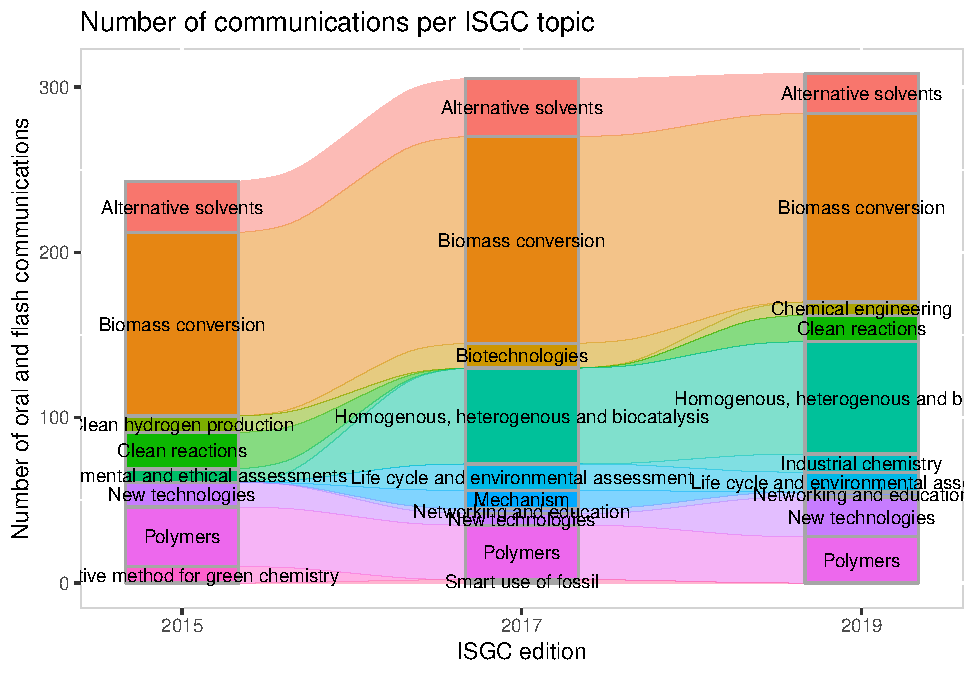
\includegraphics{ISGC_files/figure-latex/unnamed-chunk-4-1.pdf}

We observe that 4 topics are present at each edition of the congress:
Biomass conversion (named ``Renewable Carbon'' at the 2017 Edition),
Polymers, Alternative solvents, and New technologies. The 8 remaining
topics are only present at one or two editions.

\hypertarget{participation}{%
\subsection{Participation}\label{participation}}

There are different ways of approaching the conference participation. It
can be analysed using registration data or though the lens of
communications' authors i.e.~active participants. In the latter case, it
is possible to filter the information to consider only the active
participants who registered to the conference. Indeed, certain
communications' co-authors did not attend the conference.

In what follows, we consider the participation through the lens of all
communications' authors, whether they registered or not.

By counting all the speakers including industrials and keynote speakers
over the 3 editions of the congress, we find a total of 3823
participants. Among them, 154 were represented at all editions, 3211
intervened to 1 edition only, (i.e.~83.99\%), and 458 contributed to 2
editions.

If we limit ourselves to participants to oral communications and flash
communications panels, we find a total of 2366 participants. Among them,
98 were represented at all editions, 1986 intervened to 1 edition only,
(i.e.~83.94\%), and 282 contributed to 2 editions.

Overall, there had been 219 oral and flash communications distinct
panels: 64 in 2015, 78 in 2017, and 77 in 2019.

In chemistry, most communications are the result of a team work. At
ISGC, there is an average of 4.13 authors per oral and flash
communications.

\hypertarget{networks-of-panels}{%
\subsection{Networks of panels}\label{networks-of-panels}}

In each of the graphs below, the grey dots denote a Congress panel, the
blue dots denote participants who attended only one panel, and the red
dots denote `multi-positional' participants who attended more than one
Congress panel. Finally, the intensity of the links refers to an inverse
weighting that visually accentuates participation in panels with few
participants.

Remember that we are counting potential participants here: in practice,
some of these participants will not have come to the Congress.

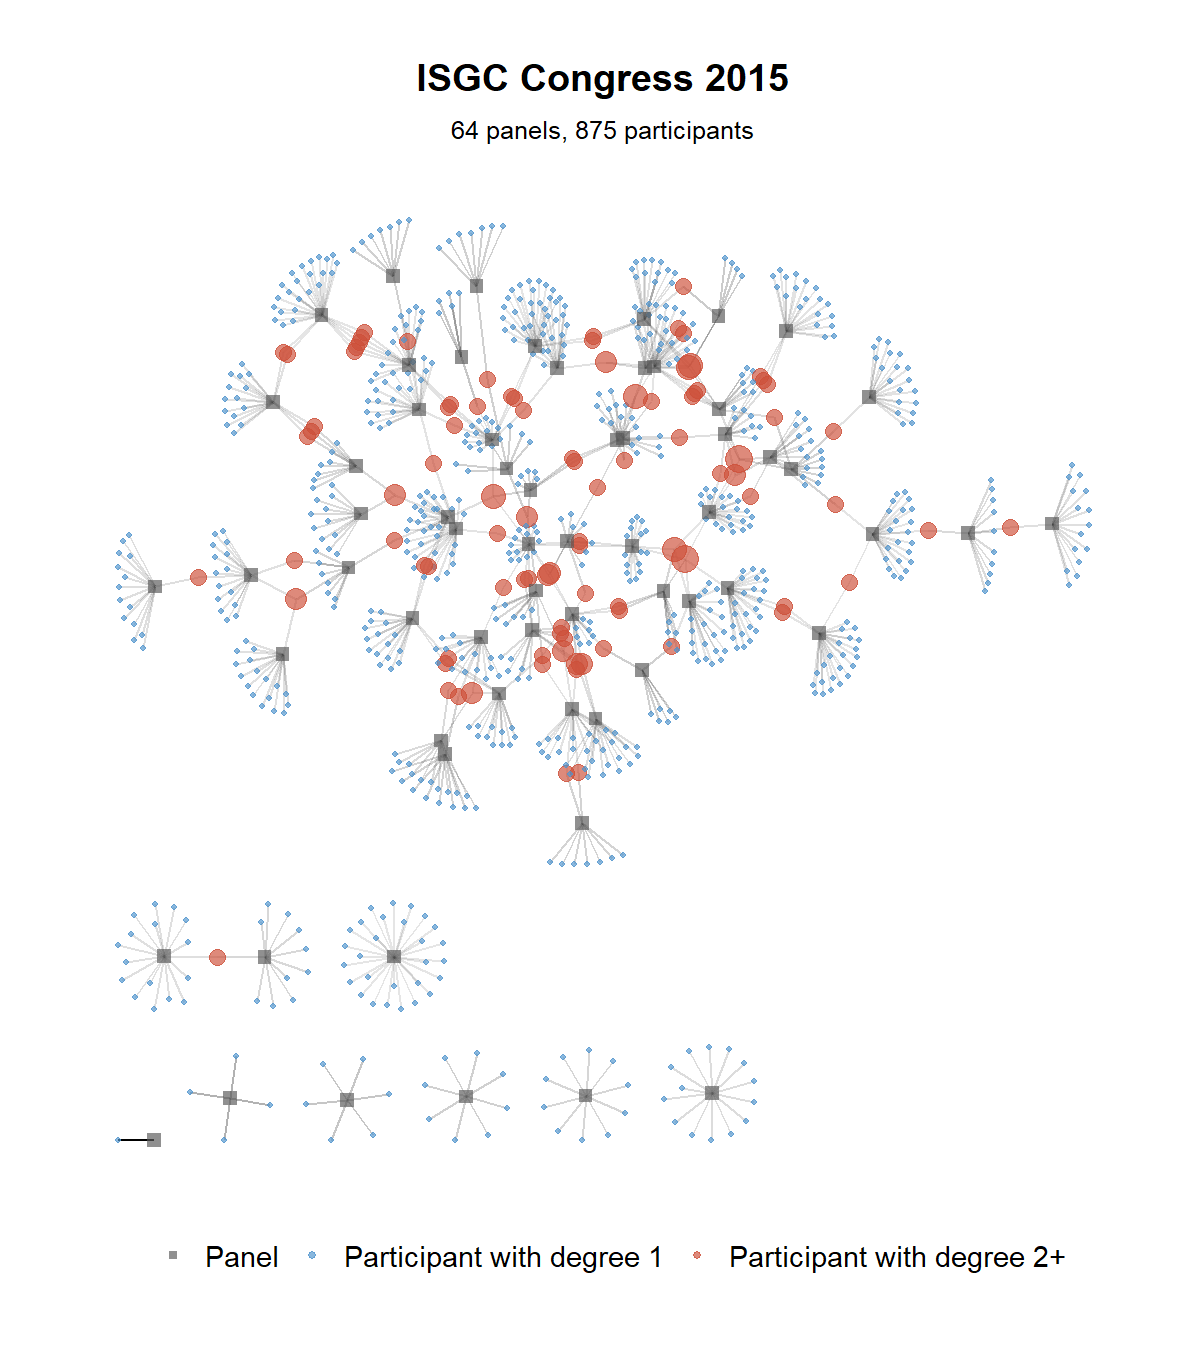
\includegraphics[width=33.33in]{plots/congres-isgc2015-2mode}
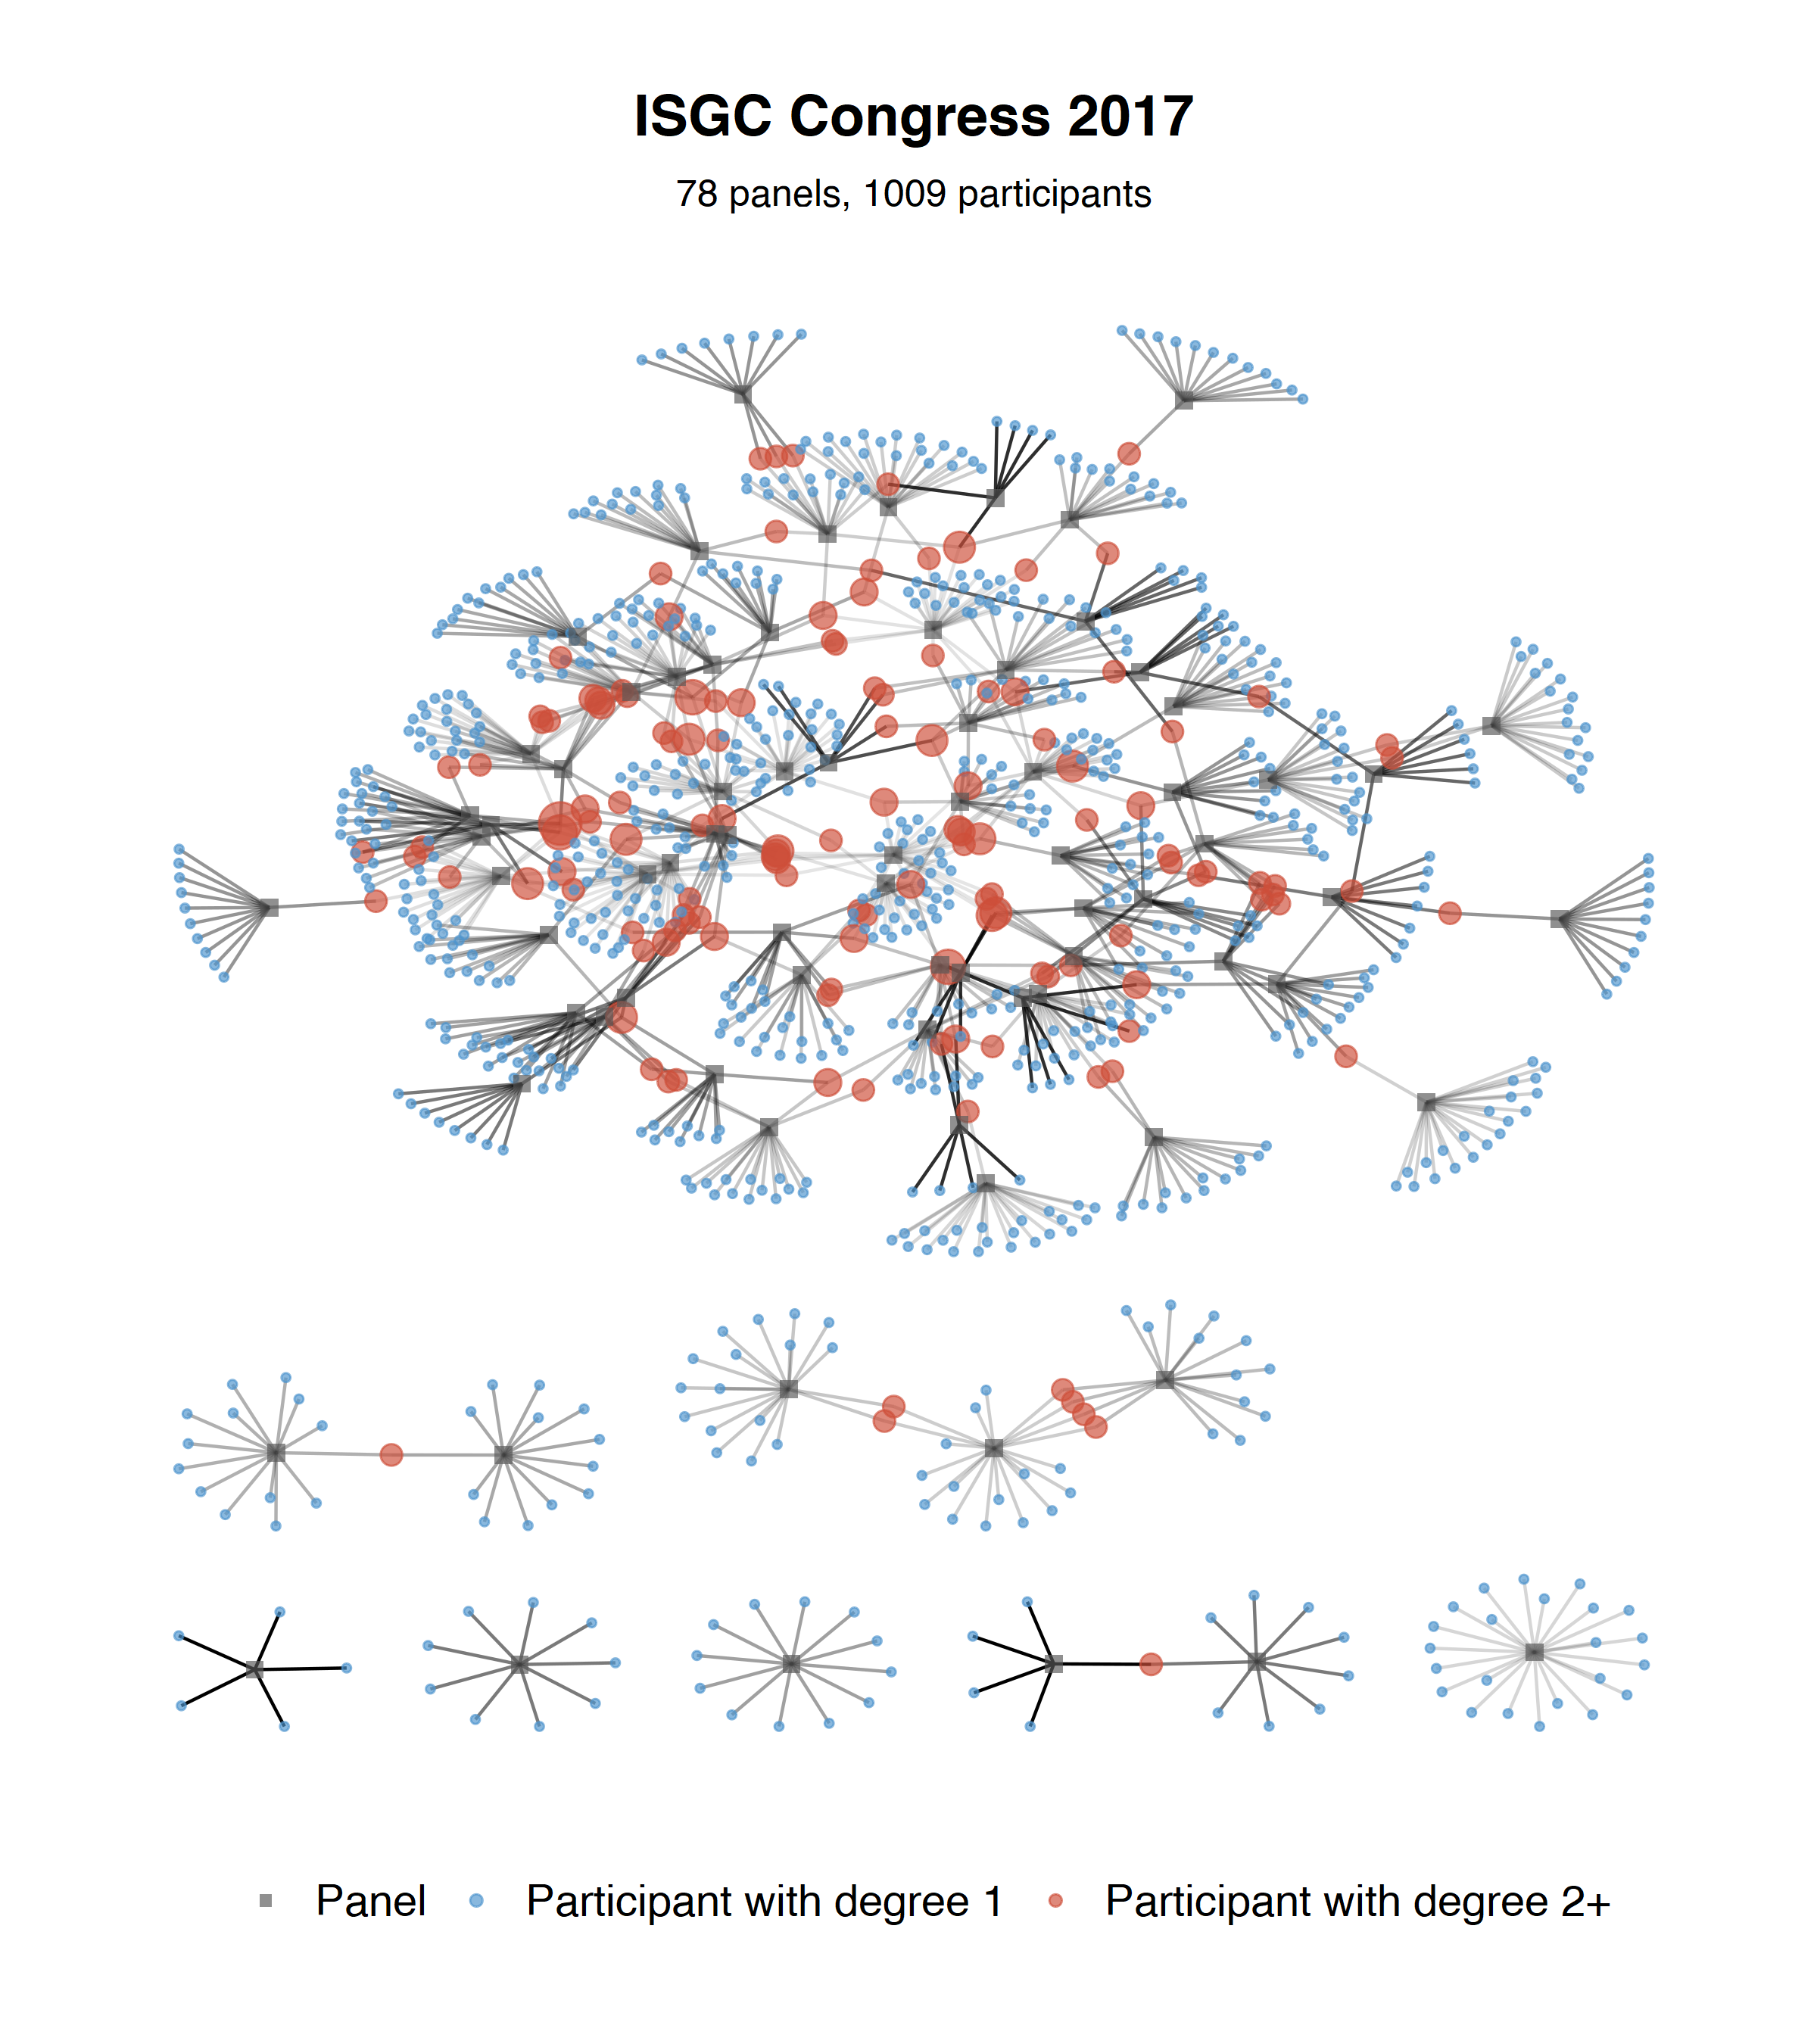
\includegraphics[width=33.33in]{plots/congres-isgc2017-2mode}
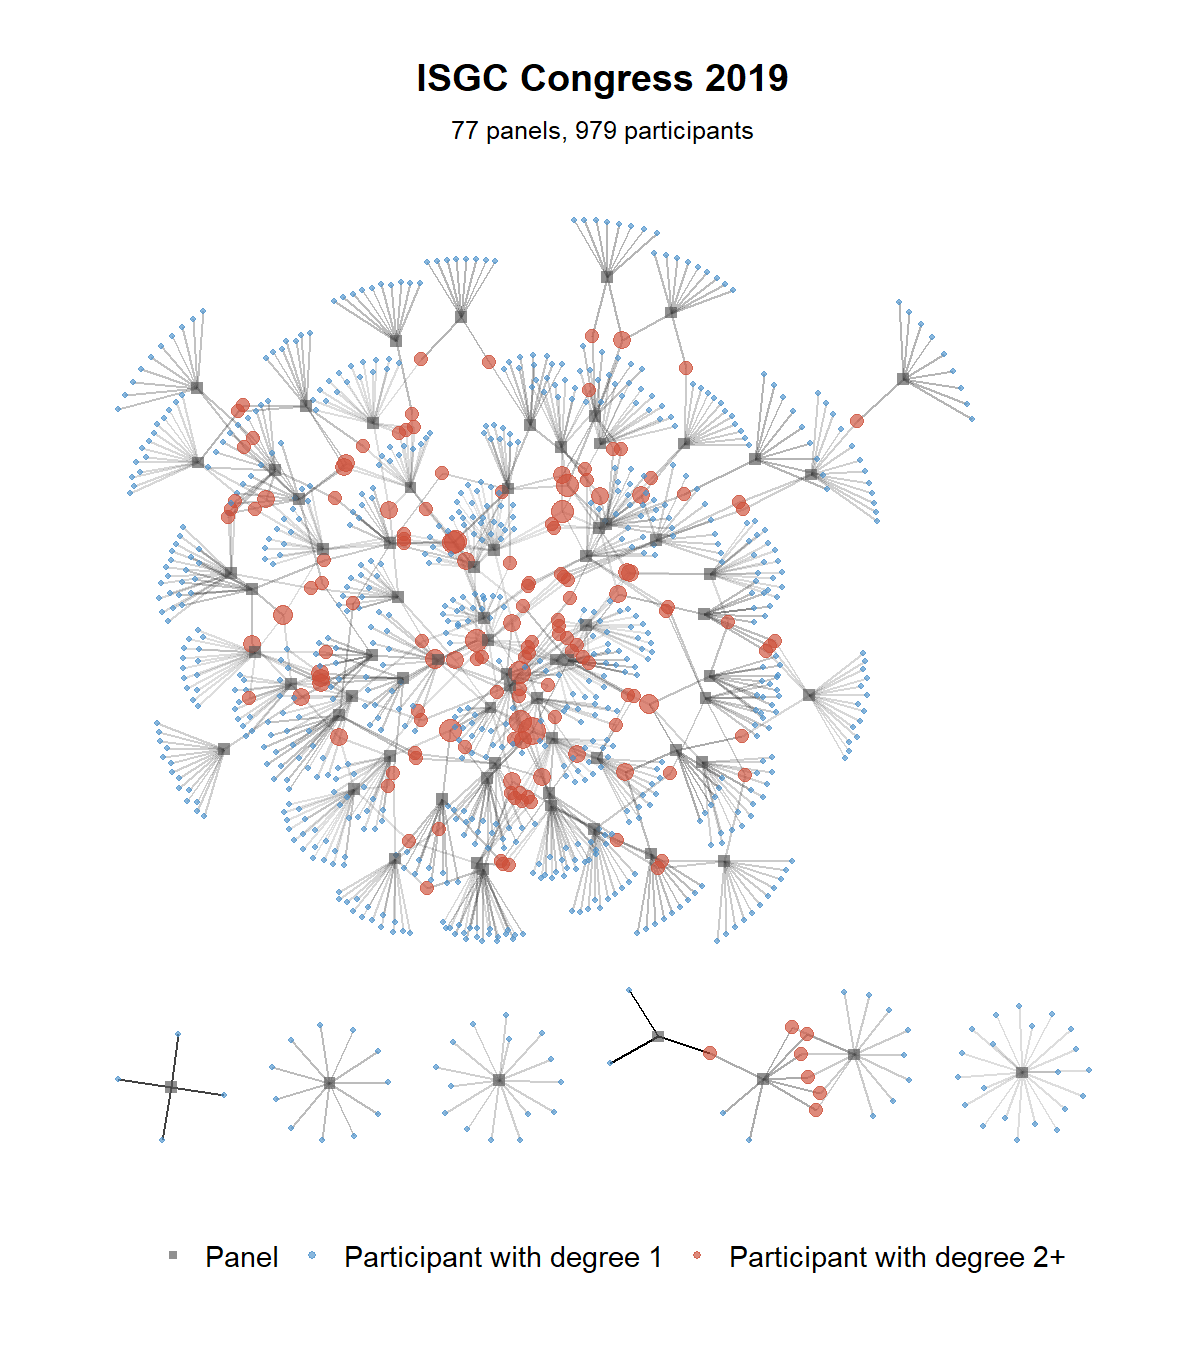
\includegraphics[width=33.33in]{plots/congres-isgc2019-2mode}

Are there more and more multi-positional participants - degree 2+ in
these bipartite graphs - at the ISGC Congress? The answer is yes,
slightly more, which can partly result from the opportunities offered by
the increased number of panels. From 2015 to 2017, the number of
multi-positional participants increased from 10.8 to 15.5\%, i.e.~an
increase of 43.52\%. At the same time, the number of panels increased
from 64 to 77, an increase of 20.31\% (see Table 2 below). The number of
multi-positional participants thus increased at a higher pace than the
number of panels.

\begin{table}
\centering
\begin{tabular}[t]{r|r|r|r|>{}r|>{}r|r}
\hline
\multicolumn{1}{c|}{ISGC Congress} & \multicolumn{1}{c|}{Panels} & \multicolumn{1}{c|}{Participants} & \multicolumn{1}{c|}{Ratio} & \multicolumn{1}{c|}{\% degree 1} & \multicolumn{1}{c|}{\% degree 2+} & \multicolumn{1}{c}{C - 1} \\
\cline{1-1} \cline{2-2} \cline{3-3} \cline{4-4} \cline{5-5} \cline{6-6} \cline{7-7}
2015 & 64 & 874 & 13.7 & 89.2 & 10.8 & 8\\
\hline
2017 & 78 & 1009 & 12.9 & \em{86.4} & \em{13.6} & 7\\
\hline
2019 & 77 & 961 & 12.5 & \em{84.5} & \em{15.5} & 4\\
\hline
\end{tabular}
\end{table}

In the table above, the ``Ratio'' column gives the ratio of participants
to panels, which drops very slightly over time. It is difficult to draw
a conclusion on the fragmentation of the conference as the number of
panels at the ISGC is the result of the organisers' choices when setting
up the programme and not of the participants. Indeed, the participants
of the ISGC congress choose to associate their paper with a main topic
and it is on this basis that the papers are then grouped into panels.

The number of isolated components of the graph, noted as ``C - 1'' above
because only components not connected to the main component have been
counted, corresponds to the number of panels in which no participant
took part in any other panel of the Congress. This figure is decreasing
over time, from 8 in 2015 to 4 in 2019, i.e.~a drop of 50\%.

In the one-mode networks below, the blue dots indicate participants who
attended only one panel of the Congress edition concerned; the red dots
indicate participants who attended several panels.

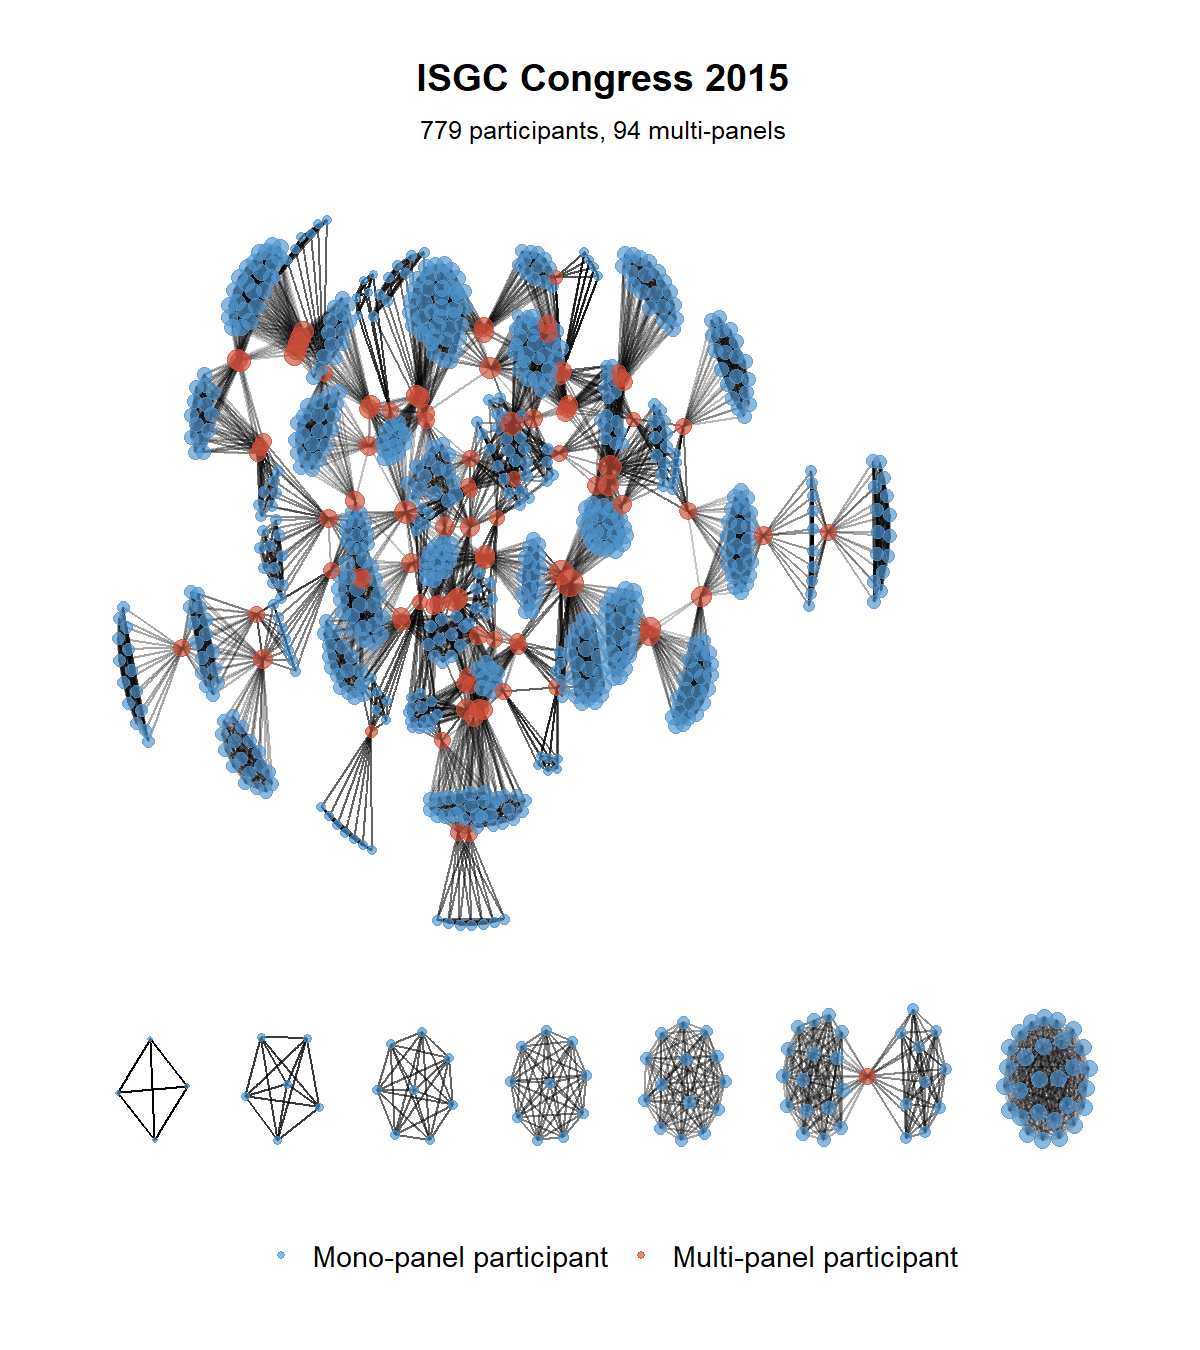
\includegraphics[width=16.67in]{plots/congres-isgc2015-1mode}
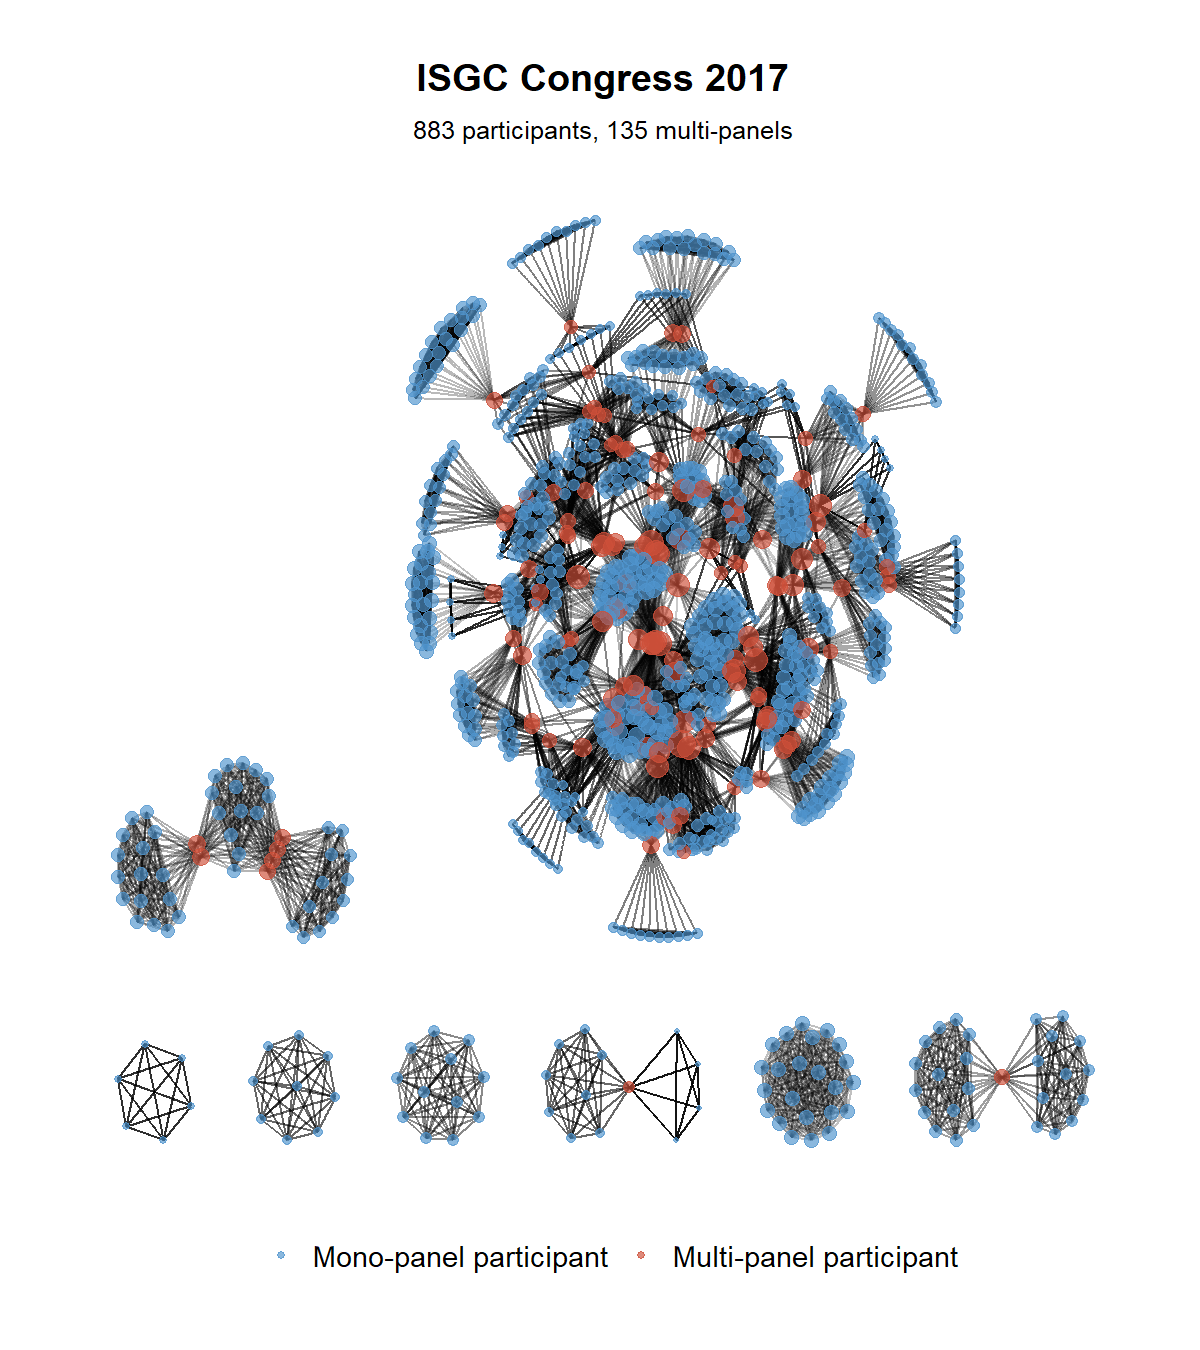
\includegraphics[width=16.67in]{plots/congres-isgc2017-1mode}
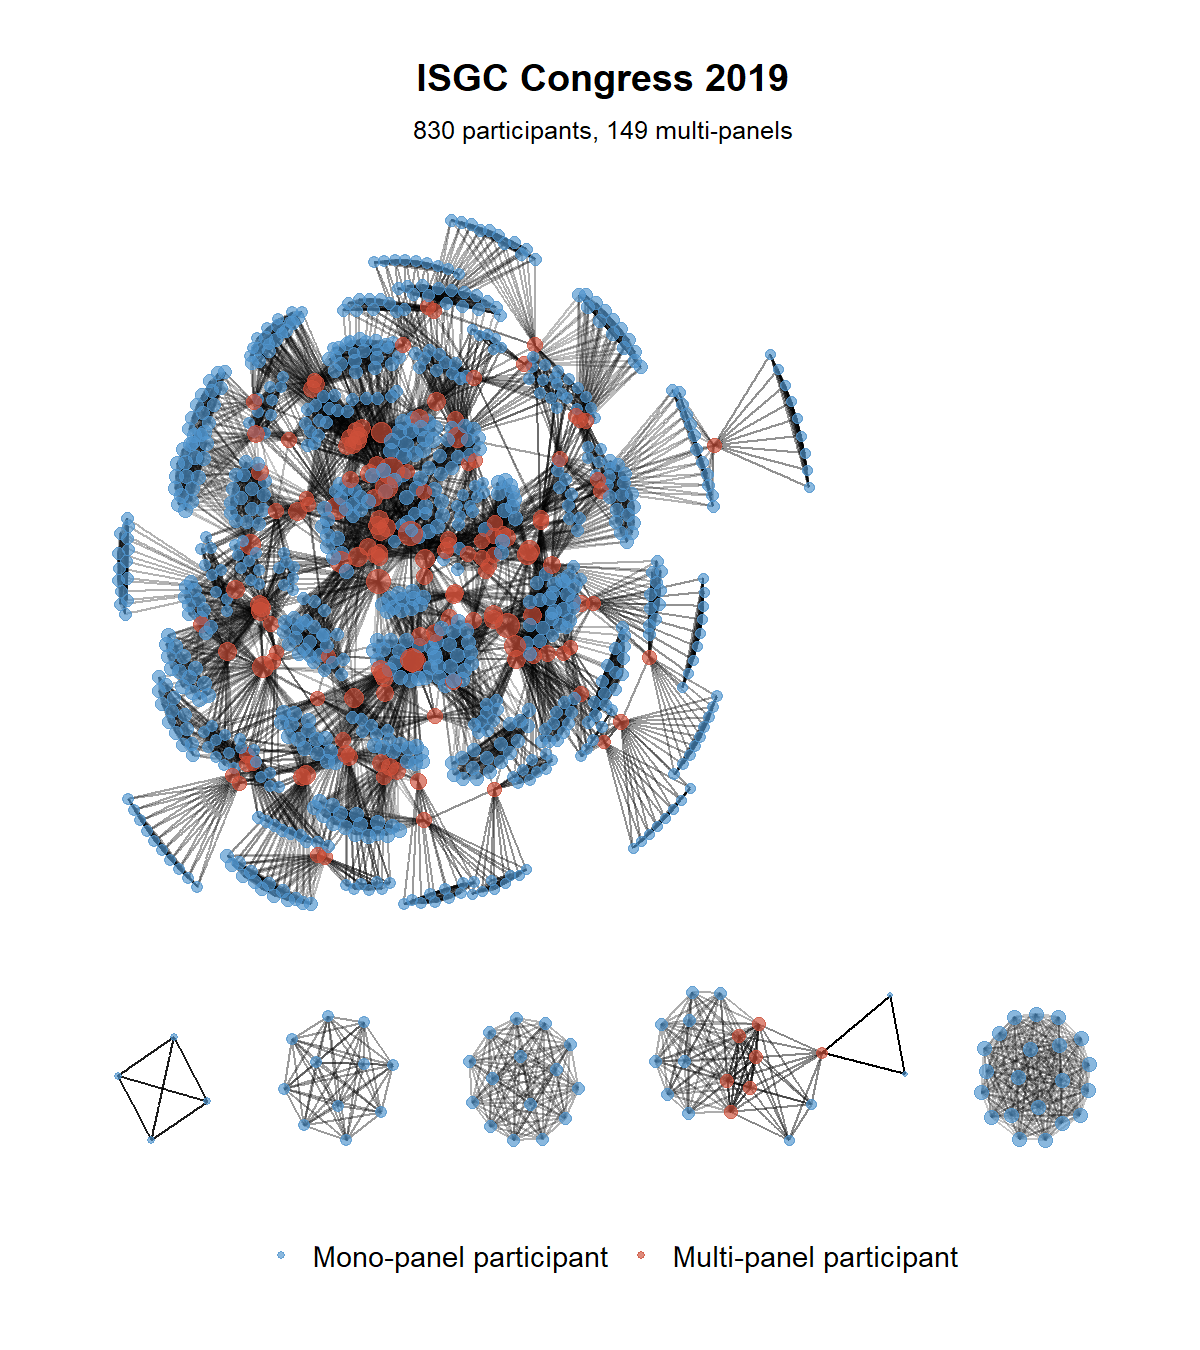
\includegraphics[width=16.67in]{plots/congres-isgc2019-1mode}

\hypertarget{linking-communications-according-to-common-authors-and-topics}{%
\subsection{Linking communications according to common authors and
topics}\label{linking-communications-according-to-common-authors-and-topics}}

We now consider the network of oral and flash communications sharing one
author at least.

\includegraphics{ISGC_files/figure-latex/unnamed-chunk-13-1.pdf}

It counts 645 communications (on a total of 856, among which 172 from
the 2015 edition, 242 from the 2017 edition, and 231 from the 2019
edition. It involves 580 participants.

There are 607 communications with different topics but at least one
common authors. We here consider the original topics' name before the
recoding suggested by François Jérôme's expertise. We group all the
communications according to their topic and attempt to visualise the
relations between topics.

\includegraphics{ISGC_files/figure-latex/unnamed-chunk-15-1.pdf}

The chord diagram with 25 different topics is not easy to read but it
confirms the important link between Biomass conservation and Renawable
Carbon that we grouped together in the 16 categories topic variable.

Since certain original topics were only present in certain editions we
attempt to visualise the relations between topics using an historical
layout. This network is derived from the network of communications
having at least one common author.

\includegraphics{ISGC_files/figure-latex/unnamed-chunk-16-1.pdf}

Let now consider the network of relations between ISGC topics using the
list of topics recoded into 16 categories.

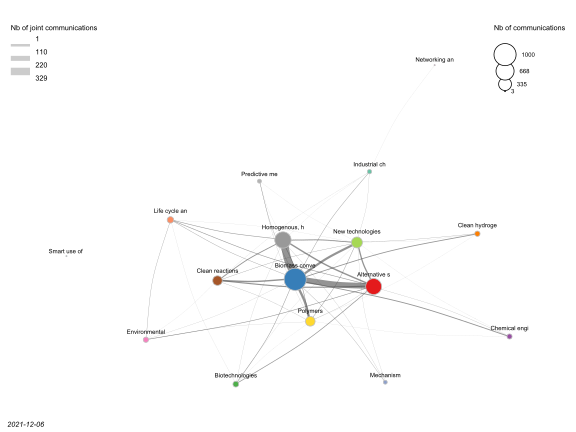
\includegraphics{plots/Topics_network_recoded_cartigraph.svg}

\hypertarget{individual-trajectory}{%
\subsection{Individual trajectory}\label{individual-trajectory}}

We focus on the specific case of PNA. A researcher who started his
career in Singapore and then moved to Poitiers, in France where he was
first hired as a postdoctoral researcher, and latter on succeeded to get
a permanent position at the CNRS. Here is a subset of the network of
communications involving this author. We notice that certain of his
co-authors are not correctly indexed in the ISGC database, which means
that we have to be very careful when interpreting coauthorship data
derived from this source.

\includegraphics{ISGC_files/figure-latex/unnamed-chunk-18-1.pdf}

\end{document}
